\documentclass[conference]{IEEEtran}
\IEEEoverridecommandlockouts
\usepackage{amsmath,amssymb}
\usepackage{graphicx}
\usepackage{booktabs}
\usepackage{multirow}
\usepackage{tikz}
\usetikzlibrary{arrows.meta,positioning,fit,calc}
\usepackage{url}
\usepackage{xcolor}
\usepackage{cite}
\usepackage[hidelinks]{hyperref}
\newcommand{\vect}[1]{\mathbf{#1}}

\begin{document}

\title{Design and Simulation of a Low-Cost Four-Beam Doppler Velocity Log with Covariance-Calibrated Beam-Level Fault Tolerance for Deep-Water INS/DVL Navigation}

\author{\IEEEauthorblockN{Tejas Jadhav}
\IEEEauthorblockA{Department of Mechatronics Engineering\\
Symbiosis Skills and Professional University, Pune, India\\
tj419306@gmail.com}}

\maketitle

\begin{abstract}
Doppler velocity logs (DVLs) are the principal velocity aid for autonomous underwater vehicle (AUV) inertial navigation, but commercial units cost several thousand US dollars and are beyond the reach of most low-cost vehicles. This paper presents the design of a four-beam, 1~MHz, narrowband DVL built from commodity components, together with a tightly coupled inertial/DVL extended Kalman filter (EKF) whose beam-level fault detection is statistically calibrated. A physically based echo model with seabed speckle shows that a single 2~ms ping is limited to about 94~Hz Doppler noise (0.07~m/s), so a realistic low-cost unit delivers 39--77~Hz per 5~Hz update rather than the 10~Hz often assumed. Under this noise the filter still bounds position error to 0.22--0.43~m over 60~s, against 15.9~m for the inertial unit alone. Normalising beam residuals by sensor noise alone, as in common practice, inflates the false-alarm rate about 30-fold at low noise; using the full innovation covariance makes healthy residuals unit-Gaussian (standard deviation 0.998). A 2-of-3 beam quarantine rule prevents the filter from absorbing persistent faults, raising isolation of a 0.05~m/s fault from 73\% to 99.95\% at 10~Hz noise. For 3800~m and 6000~m operation, uncorrected sound speed causes 1.3--3.8\% velocity scale error, which a Mackenzie-equation correction reduces to 0.15\%. The navigation error budget is dominated by the descent, not by the DVL. All results come from a reproducible Monte Carlo study; hardware validation is the subject of ongoing work.
\end{abstract}

\begin{IEEEkeywords}
Doppler velocity log, AUV navigation, INS/DVL integration, fault detection and isolation, Kalman filter, low-cost sensors, deep-sea navigation
\end{IEEEkeywords}

\section{Introduction}

AUVs navigate primarily by dead reckoning: an inertial measurement unit (IMU) propagates position and velocity, and a DVL measures velocity over the seabed to bound the drift~\cite{paull2014}. A DVL transmits acoustic pulses along four slanted beams and estimates the radial velocity of each beam from the Doppler shift of the seabed echo.

Commercial DVLs are accurate but expensive. The lowest-cost current unit, a 1~MHz Janus-array DVL rated to 300--600~m, is listed at about US\$8{,}700~\cite{wl_a50}; deep-rated units with phased arrays and broadband processing cost considerably more~\cite{tasman}. This price excludes most student, research and low-cost survey vehicles. A DVL built from commodity parts is plausible: an open-hardware, single-beam 1~MHz Doppler flow sensor has already been demonstrated for under US\$50~\cite{catsamas2022}. Such a unit, however, would have higher per-beam noise and would be more prone to beam faults than a commercial DVL.

The INS/DVL fusion literature has developed tightly coupled filters that use raw beam measurements and remain usable when beams are lost~\cite{tal2017,liu2018,yao2023,klein2020,klein2022,yona2023,cohen2024}. Fault detection, however, has been treated heuristically or with fixed noise models and evaluated mainly in simulation~\cite{zhu2025,yang2022}, without calibrated false-alarm rates. All of this work assumes commercial-grade sensors.

\subsection{Problem Statement}

It is not known whether tightly coupled INS/DVL navigation and beam-level fault detection remain reliable when the DVL is a low-cost, narrowband unit with several times higher noise than commercial sensors, nor how detection thresholds should be set so that false alarms match their design value. It is also not known what limits such a design if it is made pressure-tolerant for deep operation.

\subsection{Contributions}
\begin{enumerate}
\item A complete design of a four-beam, 1~MHz DVL from commodity components, with the acoustic, signal-processing and timing calculations that set its achievable precision (Sections~\ref{sec:design}--\ref{sec:measurement}).
\item A quantification of the noise such a unit can actually deliver, and of how navigation and fault detection degrade under it (Section~\ref{sec:nav}).
\item A demonstration that normalising beam residuals by sensor noise alone inflates false alarms about 30-fold, and that the full innovation covariance restores the design value (Section~\ref{sec:fdi}).
\item A 2-of-3 quarantine rule that prevents fault absorption, with isolation maps against fault size and noise (Section~\ref{sec:fdi}).
\item A deep-water (3800 and 6000~m) error budget covering sound speed, bottom-lock range, descent drift and pressure housing (Section~\ref{sec:deep}).
\end{enumerate}

\section{Related Work}

\emph{Low-cost Doppler sensing.} Catsamas \emph{et~al.}~\cite{catsamas2022} built an open-hardware 1~MHz continuous-wave Doppler water-velocity sensor using an SA612 mixer and an 8-bit microcontroller, with errors up to $\pm$11\% above 0.4~m/s. It is single-beam and fixed, and does no bottom tracking. Blanford \emph{et~al.}~\cite{blanford2018} studied design trade-offs for compact correlation velocity logs, and Rypkema~\cite{rypkema2019} proposed passive inverted USBL to avoid the DVL altogether on low-cost vehicles. We found no published open, four-beam, bottom-tracking DVL design.

\emph{Tightly coupled fusion and missing beams.} Loosely coupled fusion requires at least three beams to form a 3-D velocity. Tal \emph{et~al.}~\cite{tal2017} extended it with virtual beams. Liu \emph{et~al.}~\cite{liu2018} fused raw beams with pressure depth in a tightly coupled filter, and Yao \emph{et~al.}~\cite{yao2023} built virtual beams inside one. Klein and co-authors estimated velocity during complete outages~\cite{klein2020,klein2022}, and learning-based methods regress missing beams from past data~\cite{yona2023,cohen2024}. These works assume commercial DVLs with per-beam noise of a few mm/s.

\emph{Fault detection.} Zhu \emph{et~al.}~\cite{zhu2025} detect beam faults by Janus-pair symmetry and innovation jumps, then inflate the faulty beam's noise or rebuild it by grey prediction; detection was not tested independently. Yang \emph{et~al.}~\cite{yang2022} used a robust interacting-multiple-model filter. Neither reports a calibrated false-alarm rate. In GNSS/INS integrity, Quartararo and Langel~\cite{quartararo2022} showed that a filter which keeps ingesting a fault ``begins to follow the faulty state trajectory'', which lowers detection probability. We show the same effect for single DVL beams and give a simple remedy.

\emph{Deep-water navigation.} Autosub6000 descended at 0.9~m/s to 4600~m with a 300~kHz DVL that tracked the seabed only within 220~m, and needed acoustic range fixes to correct its position after descent~\cite{mcphail2008}. Deep-sea trials report USBL errors of about 80~m at 4000~m depth~\cite{liu2024}.

\section{DVL Design}
\label{sec:design}

\subsection{Architecture}

Fig.~\ref{fig:block} shows the proposed design. The hardware has not yet been built; the parameters below define the design and are the inputs to the simulations in Sections~\ref{sec:measurement}--\ref{sec:deep}.

\begin{figure*}[t]
\centering
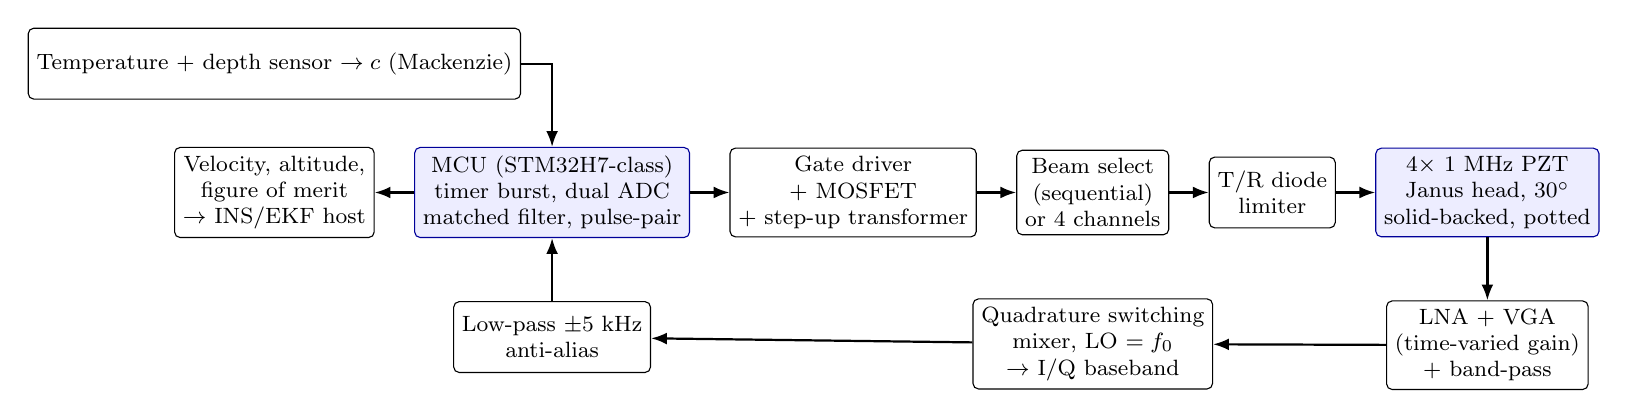
\begin{tikzpicture}[font=\footnotesize, node distance=5mm and 5mm,
  blk/.style={draw, rounded corners=2pt, align=center, minimum height=9mm, inner sep=3pt},
  acc/.style={blk, fill=blue!7, draw=blue!60!black},
  ar/.style={-{Latex[length=2mm]}, thick}]
\node[acc] (mcu) {MCU (STM32H7-class)\\timer burst, dual ADC\\matched filter, pulse-pair};
\node[blk, left=of mcu] (out) {Velocity, altitude,\\figure of merit\\$\rightarrow$ INS/EKF host};
\node[blk, right=of mcu] (drv) {Gate driver\\+ MOSFET\\+ step-up transformer};
\node[blk, right=of drv] (mux) {Beam select\\(sequential)\\or 4 channels};
\node[blk, right=of mux] (tr) {T/R diode\\limiter};
\node[acc, right=of tr] (xd) {4$\times$ 1~MHz PZT\\Janus head, 30$^\circ$\\solid-backed, potted};
\node[blk, below=8mm of mcu] (lpf) {Low-pass $\pm$5~kHz\\anti-alias};
\node[blk, below=8mm of mux] (mix) {Quadrature switching\\mixer, LO $=f_0$\\$\rightarrow$ I/Q baseband};
\node[blk, below=8mm of xd] (lna) {LNA + VGA\\(time-varied gain)\\+ band-pass};
\node[blk, above=6mm of out] (env) {Temperature + depth sensor $\rightarrow c$ (Mackenzie)};
\draw[ar] (mcu) -- (out); \draw[ar] (mcu) -- (drv); \draw[ar] (drv) -- (mux); \draw[ar] (mux) -- (tr); \draw[ar] (tr) -- (xd);
\draw[ar] (xd) -- (lna); \draw[ar] (lna) -- (mix); \draw[ar] (mix) -- (lpf); \draw[ar] (lpf) -- (mcu);
\draw[ar] (env.east) -| (mcu.north);
\end{tikzpicture}
\caption{Proposed low-cost DVL. Shaded blocks are the transducer head and the processor. A single receive chain shared sequentially by the four beams is the minimum build; four parallel chains halve the noise (Section~\ref{sec:nav}).}
\label{fig:block}
\end{figure*}

\subsection{Transducers and Beam Geometry}

Four piezoceramic (PZT) discs operate at $f_0=1$~MHz. In seawater with $c\approx1500$~m/s the wavelength is $\lambda=c/f_0=1.5$~mm. For a circular piston of diameter $D$, the full $-3$~dB beamwidth is approximately
\begin{equation}
\theta_{3\mathrm{dB}} \approx 1.02\,\frac{\lambda}{D},
\end{equation}
so $D=20$~mm gives $\theta_{3\mathrm{dB}}\approx0.077$~rad $=4.4^\circ$. The near-field (Fraunhofer) distance $D^2/(4\lambda)=67$~mm is far below the operating altitude. The discs are mounted in a Janus configuration at $\theta=30^\circ$ from vertical, giving unit beam vectors (body frame, $z$ down)
\begin{equation}
\vect{B}=\begin{bmatrix}\vect b_1^\top\\ \vect b_2^\top\\ \vect b_3^\top\\ \vect b_4^\top\end{bmatrix}
=\begin{bmatrix} s&0&c_\theta\\ -s&0&c_\theta\\ 0&s&c_\theta\\ 0&-s&c_\theta\end{bmatrix},\quad s=\sin\theta,\ c_\theta=\cos\theta .
\end{equation}
For deep operation the discs are backed with solid particle-filled epoxy rather than air, so the head contains no voids (Section~\ref{sec:deep}).

\subsection{Transmit and Receive Chain}

A microcontroller timer generates a 2~ms tone burst (2000 cycles), giving a range resolution of $c\tau/2=1.5$~m. A gate driver and MOSFET stage with a step-up transformer drives the selected disc; a series-resistor and diode limiter protects the receiver. The echo passes through a low-noise amplifier and a variable-gain amplifier with time-varied gain to compensate spreading loss.

A quadrature switching mixer with local oscillator at $f_0$ shifts the echo to complex baseband, as in~\cite{catsamas2022}. The Doppler shift of beam $i$ is
\begin{equation}
f_{D,i}=\frac{2f_0}{c}\,v_{r,i},\qquad v_{r,i}=\vect b_i^\top\vect v ,
\label{eq:doppler}
\end{equation}
so a radial velocity of 0.5~m/s gives 666.7~Hz, and $\pm3$~m/s maps to $\pm4$~kHz. A $\pm5$~kHz low-pass filter and 40~kS/s sampling of I and Q by the microcontroller's dual ADC therefore capture all expected Doppler shifts without sampling the 1~MHz carrier directly.

\subsection{Ping Timing}

At altitude $h$ the slant range is $R=h/\cos\theta$. With pulse length $\tau$ and a guard interval $\tau_g$, one ping cycle lasts
\begin{equation}
T_{\mathrm{ping}}=\frac{2R}{c}+\tau+\tau_g .
\end{equation}
At $h=20$~m, $R=23.1$~m and $T_{\mathrm{ping}}=33.8$~ms (with $\tau_g=1$~ms). At a 5~Hz update rate, each beam receives $n=(1/f_u)/T_{\mathrm{ping}}=5.9$ pings with four parallel receive chains, or $n/4=1.48$ pings when one chain is shared sequentially.

\subsection{Sound-Speed Compensation}

Since (\ref{eq:doppler}) scales with $c$, an onboard temperature and depth sensor feeds the Mackenzie equation~\cite{mackenzie1981} to estimate $c$ at the transducer (Section~\ref{sec:deep}).

\section{Measurement Model and Echo Processing}
\label{sec:measurement}

\subsection{Velocity Reconstruction and Observability}

With per-beam radial noise $\sigma_r=c\,\sigma_f/(2f_0)$, a 10~Hz Doppler noise maps to $\sigma_r=0.0075$~m/s (Monte Carlo: 0.0075~m/s). The least-squares velocity
\begin{equation}
\hat{\vect v}=(\vect B^\top\vect B)^{-1}\vect B^\top\vect v_r
\end{equation}
has standard deviations $\sigma_r/(\sqrt2\sin\theta)$ horizontally and $\sigma_r/(2\cos\theta)$ vertically. At $30^\circ$ these are 0.0106 and 0.0043~m/s (Monte Carlo: 0.01065, 0.01059, 0.00433~m/s). Any three beams keep $\mathrm{rank}(\vect B)=3$, with condition number rising from 2.45 to 3.82; two beams give rank 2, so 3-D velocity is unobservable from the DVL alone.

\subsection{Seabed Echo Model}

The baseband echo of one beam is modelled as the sum of $N_s=300$ seabed scatterers drawn across a Gaussian two-way beam pattern of $4^\circ$ width:
\begin{equation}
x(t)=\sum_{k=1}^{N_s}a_k\,w(t-\tau_k)\,e^{\,j(2\pi f_k t+\phi_k)}+n(t),
\end{equation}
where $a_k$ is complex Gaussian, $\tau_k=2R_k/c$ and $f_k=2f_0\,\vect u_k^\top\vect v/c$ depend on each scatterer's direction $\vect u_k$, $w$ is the tapered pulse envelope and $n$ is complex white noise. Scatterers at different angles produce different delays and Doppler shifts, which creates speckle and Doppler spread.

\subsection{Estimators}

Range is estimated by an energy (incoherent) matched filter, which is insensitive to the unknown Doppler phase:
\begin{equation}
y[n]=\sum_m |x[n+m]|^2\,w[m],\qquad \hat h=\frac{c\,\hat t}{2}\cos\theta ,
\end{equation}
with $\hat t$ the time of the peak of $y$. Doppler is estimated by the pulse-pair method from the gated echo, using the autocorrelation at lag $L$:
\begin{equation}
R(L)=\sum_n x[n+L]\,x^*[n],\qquad \hat f_L=\frac{f_s}{2\pi L}\left(\angle R(L)+2\pi m\right).
\label{eq:pp}
\end{equation}
Lag 1 is unambiguous to $\pm f_s/2=\pm20$~kHz but noisy; lag $L=8$ is more precise but ambiguous beyond $\pm2.5$~kHz. The dual-lag estimator picks the integer $m$ that brings $\hat f_8$ closest to $\hat f_1$. It needs two complex sums per ping, against an 8192-point FFT for a zero-padded spectral estimator.

\subsection{Results}

Fig.~\ref{fig:a3} shows single-ping precision from 300 Monte Carlo pings per point at 20~m altitude and $\vect v=[1.0,0.4,0.2]^\top$~m/s. Speckle sets a floor of about 0.07~m/s even at high SNR: 94~Hz for dual-lag pulse-pair at 20~dB. The FFT and dual-lag estimators reach the same floor, while lag-1 pulse-pair degrades badly at low SNR (0.24~m/s at 0~dB). Altitude error is 0.21~m RMS at 20~m. Reaching 10~Hz would require averaging $(94/10)^2\approx89$ pings per beam, more than the timing of Section~\ref{sec:design} allows at 5~Hz.

\begin{figure}[t]
\centering
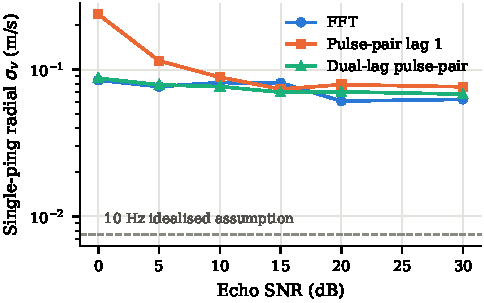
\includegraphics[width=\columnwidth]{fig/a3_precision.pdf}
\caption{Single-ping radial velocity precision versus echo SNR, speckled seabed echo, 300 Monte Carlo pings per point.}
\label{fig:a3}
\end{figure}

\section{Tightly Coupled INS/DVL Navigation}
\label{sec:nav}

\subsection{Filter}

The EKF state is $\vect x=[\vect p^\top,\vect v^\top,\vect b_a^\top]^\top$ (position, velocity, accelerometer bias). With IMU specific force $\vect a_m$ at interval $\Delta t$, the prediction is
\begin{align}
\vect p_{k+1}&=\vect p_k+\vect v_k\Delta t+\tfrac12(\vect a_m-\vect b_a)\Delta t^2,\nonumber\\
\vect v_{k+1}&=\vect v_k+(\vect a_m-\vect b_a)\Delta t,\\
\vect P_{k+1}&=\vect F\vect P_k\vect F^\top+\vect G\vect G^\top\sigma_a^2+\vect Q_b ,\nonumber
\end{align}
with $\vect G=[\tfrac12\Delta t^2\vect I,\ \Delta t\vect I,\ \vect 0]^\top$. Each beam is a scalar measurement $z_i=\vect b_i^\top\vect v+n_i$ with $\vect H_i=[\vect 0,\ \vect b_i^\top,\ \vect 0]$, applied by sequential updates. A single beam therefore still constrains velocity along its own direction.

Simulation parameters: IMU at 100~Hz, $\sigma_a=0.02$~m/s$^2$ per sample, per-axis bias $\sigma_b=0.005$~m/s$^2$ ($\approx0.5$~mg), DVL at 5~Hz, a 60~s three-axis manoeuvre, and 100--200 Monte Carlo runs per case.

\subsection{Results}

\emph{DVL aiding.} With idealised 10~Hz Doppler noise, final position RMSE falls from 15.91~m (IMU only) to 0.059~m, and velocity RMSE from 0.518 to 0.0049~m/s (Fig.~\ref{fig:b1}). Without bias states, the same filter reaches 60.3~m and its normalised residuals have standard deviation 50.9 instead of 1.0, so bias estimation is essential for both accuracy and consistency.

\begin{figure}[t]
\centering
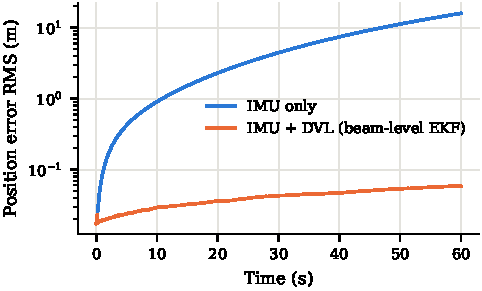
\includegraphics[width=\columnwidth]{fig/b1_drift.pdf}
\caption{Position error RMS, IMU only versus IMU+DVL beam-level EKF (200 Monte Carlo runs, 10~Hz Doppler noise).}
\label{fig:b1}
\end{figure}

\emph{Dropout and outages.} Random dropout of 50\% of beam measurements raises final position RMSE only to 0.078~m. During a full 30~s outage, position error grows to 0.30~m. After the DVL returns, velocity error recovers within about 1~s (0.0059~m/s), but position settles at 0.22~m and does not return to its pre-outage level (Fig.~\ref{fig:b2}). A DVL observes velocity, not position, so drift accumulated during an outage is permanent.

\begin{figure}[t]
\centering
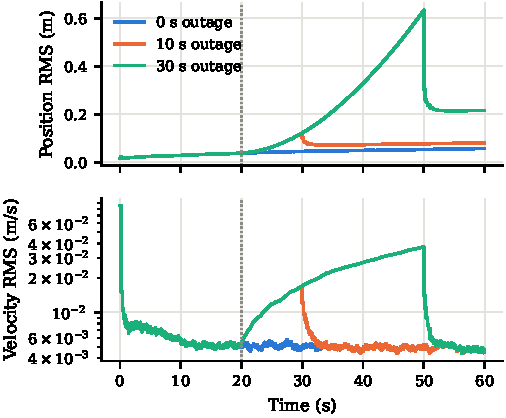
\includegraphics[width=\columnwidth]{fig/b2_outage.pdf}
\caption{Effect of DVL outages beginning at $t=20$~s. Velocity recovers within about 1~s; position error accumulated during the outage remains.}
\label{fig:b2}
\end{figure}

\emph{Update rate.} Final position RMSE falls from 0.120~m at 1~Hz to 0.040~m at 10~Hz, and is the same for bias levels from 0.001 to 0.02~m/s$^2$ once bias is estimated.

\emph{Realistic low-cost noise.} Averaging $n$ pings gives $\sigma_f=94/\sqrt n$~Hz. Table~\ref{tab:b5} applies the ping counts of Section~\ref{sec:design}. A low-cost unit delivers 39--77~Hz at 5~Hz, four to eight times the idealised value. Position error after 60~s rises to 0.22--0.43~m, still about 40 times better than the IMU alone. Four parallel receive chains halve the noise relative to one shared chain, and are the most effective hardware upgrade.

\begin{table}[t]
\centering
\caption{Navigation with the noise a low-cost DVL can deliver (20~m altitude, 60~s, 100 runs)}
\label{tab:b5}
\setlength{\tabcolsep}{3pt}
\footnotesize
\begin{tabular}{lcccc}
\toprule
Chains, rate & Pings/beam & Noise (Hz) & Pos. (m) & Vel. (m/s)\\
\midrule
1 shared, 5 Hz & 1.48 & 77.3 & 0.433 & 0.0170\\
1 shared, 2 Hz & 3.70 & 48.9 & 0.384 & 0.0164\\
4 parallel, 5 Hz & 5.92 & 38.6 & 0.216 & 0.0107\\
4 parallel, 2 Hz & 14.8 & 24.4 & 0.194 & 0.0099\\
Idealised, 5 Hz & -- & 10.0 & 0.059 & 0.0047\\
\bottomrule
\end{tabular}
\end{table}

\emph{Permanent beam failures.} Table~\ref{tab:c3} lists beams lost permanently at $t=10$~s. Losing one beam barely matters. With two opposite beams (1, 2) left out, only the $y$ axis, which no remaining beam observes, drifts (1.13~m), while $x$ and $z$ stay at the centimetre level. Because each surviving beam constrains its own direction, the tightly coupled filter degrades gradually instead of failing once fewer than three beams remain.

\begin{table}[t]
\centering
\caption{Final position RMSE (m) after permanent beam loss}
\label{tab:c3}
\begin{tabular}{lcccc}
\toprule
Beams lost & 3-D & $x$ & $y$ & $z$\\
\midrule
None & 0.056 & 0.039 & 0.037 & 0.017\\
1 (beam 1) & 0.073 & 0.060 & 0.037 & 0.020\\
2 opposite (1, 2) & 1.127 & 1.126 & 0.037 & 0.020\\
2 adjacent (1, 3) & 1.116 & 0.735 & 0.726 & 0.422\\
3 (1, 2, 3) & 1.594 & 1.126 & 0.976 & 0.566\\
All 4 & 1.978 & 1.126 & 1.253 & 1.036\\
\bottomrule
\end{tabular}
\end{table}

\section{Calibrated Beam-Level Fault Detection}
\label{sec:fdi}

\subsection{Normalised Residual Test}

Before each update, the residual of beam $i$ is $r_i=z_i-\vect b_i^\top\hat{\vect v}^-$, and its predicted variance is the scalar innovation covariance
\begin{equation}
S_i=\vect b_i^\top\vect P_v^-\vect b_i+\sigma_r^2 ,
\label{eq:Si}
\end{equation}
where $\vect P_v^-$ is the prior velocity covariance at that epoch. The beam is flagged when $|z_i|=|r_i|/\sqrt{S_i}>k$. For a consistent filter $z_i\sim\mathcal N(0,1)$~\cite{barshalom2001}, so the false-alarm probability per beam-epoch is
\begin{equation}
P_{\mathrm{FA}}=\mathrm{erfc}\!\left(k/\sqrt2\right),
\end{equation}
which is $6.3\times10^{-5}$ for $k=4$. A common simplification normalises by $\sigma_r$ alone, ignoring the first term of (\ref{eq:Si}).

\subsection{Quarantine Rule}

A flagged beam is rejected at that epoch. If the beam is flagged in at least 2 of the last 3 epochs, it is treated as persistently faulty and excluded for a hold time of 2~s, renewed while it keeps failing. A single outlier therefore costs one measurement, while a persistent fault is kept out even if it occasionally passes the test.

\subsection{Results}

\emph{Calibration.} Fig.~\ref{fig:c1} shows healthy residuals over 200 runs at 10~Hz noise: with (\ref{eq:Si}) they have standard deviation 0.998 and follow $\mathcal N(0,1)$. Across noise levels from 2 to 40~Hz the empirical 4$\sigma$ false-alarm rate stays between $0.7\times10^{-4}$ and $1.1\times10^{-4}$, close to the design value of $6.3\times10^{-5}$. Normalising by $\sigma_r$ alone inflates the standard deviation to 1.31 at 2~Hz noise and the 4$\sigma$ false-alarm rate from 0.0076\% to 0.23\%, about 30-fold. The error shrinks as sensor noise grows, because the neglected INS term becomes relatively smaller. This is consistent with the high low-noise false-alarm rates observed in our earlier exploratory experiments.

\begin{figure*}[t]
\centering
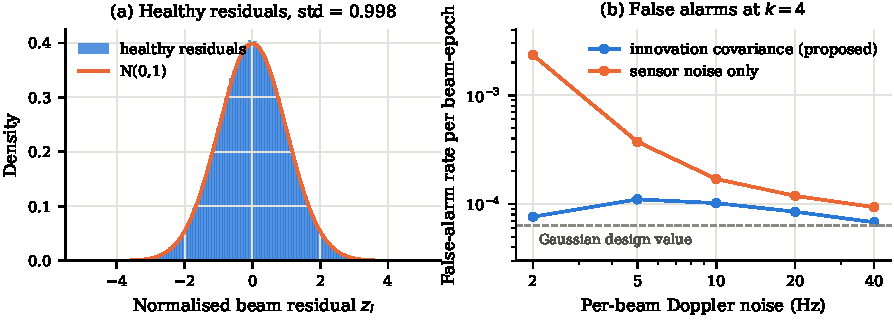
\includegraphics[width=0.85\textwidth]{fig/c1_calibration.pdf}
\caption{(a) Healthy normalised beam residuals with the innovation covariance (\ref{eq:Si}), 10~Hz noise, 200 runs. (b) 4$\sigma$ false-alarm rate versus sensor noise for the two normalisations.}
\label{fig:c1}
\end{figure*}

\emph{Isolation and absorption.} A step bias was added to one random beam from $t=30$~s (Fig.~\ref{fig:c2}). Without quarantine, isolation of a 0.05~m/s fault at 10~Hz noise is only 73\%: each missed epoch lets the filter absorb part of the fault into its velocity and bias estimates, which shrinks later residuals. With quarantine it rises to 99.95\%. The smallest fault isolated at least 95\% of the time is 0.03, 0.05 and 0.10~m/s at 5, 10 and 20~Hz noise, or about 6.7--8$\sigma_r$. A 0.1~m/s fault left undetected produces 3.13~m of final position error; with detection the error is 0.070~m. At the realistic noise of Table~\ref{tab:b5} the isolation threshold scales to roughly 0.19--0.39~m/s.

\begin{figure}[t]
\centering
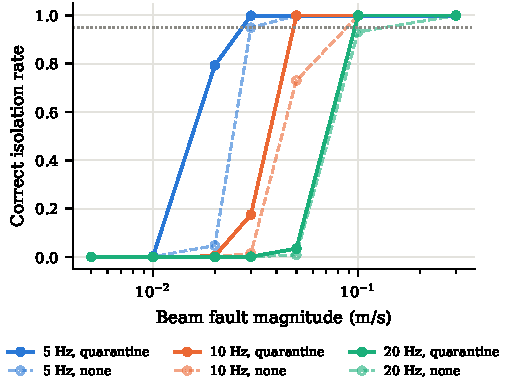
\includegraphics[width=\columnwidth]{fig/c2_isolation.pdf}
\caption{Correct isolation of a single-beam step fault ($k=4$, 100 runs per point). Dashed: same detector without quarantine. Dotted line: 95\%.}
\label{fig:c2}
\end{figure}

\emph{Outliers and intermittent faults.} With 2\% gross outliers ($\pm0.5$~m/s), fault detection reduces final position RMSE from 0.491 to 0.059~m while discarding only 0.9\% of healthy data, with a true false-alarm rate of 0.01\%. For an intermittent 0.1~m/s fault (2~s on, 5~s period), error falls from 2.10 to 0.068~m; 9.1\% of healthy epochs are excluded, because the quarantine keeps the unreliable beam out between faulty spells.

\section{Deep-Water Analysis: 3800~m and 6000~m}
\label{sec:deep}

\subsection{Environment and Sound Speed}

Sound speed follows Mackenzie~\cite{mackenzie1981} and absorption follows Francois and Garrison~\cite{francois1982}, for a tropical profile with a 28$^\circ$C mixed layer to 50~m decaying to about 1.5$^\circ$C at depth, and salinity 35 (Fig.~\ref{fig:d1}). Pressure is 38.3~MPa at 3800~m and 60.4~MPa at 6000~m, where sound speed is 1520.1 and 1559.3~m/s.

\begin{figure*}[t]
\centering
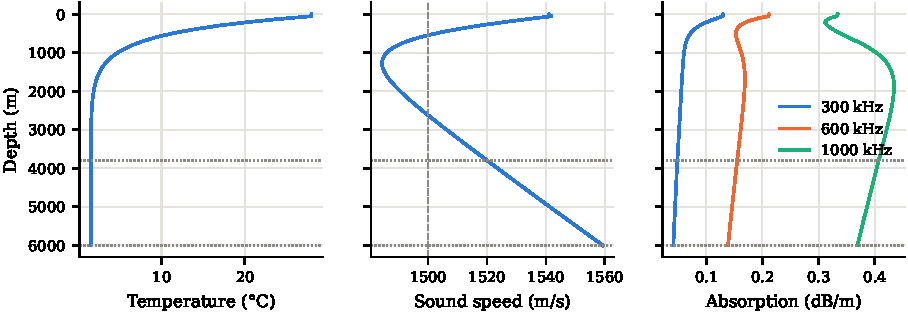
\includegraphics[width=0.85\textwidth]{fig/d1_environment.pdf}
\caption{Assumed temperature profile, resulting sound speed (dashed: 1500~m/s) and absorption at 300, 600 and 1000~kHz. Dotted lines mark 3800 and 6000~m.}
\label{fig:d1}
\end{figure*}

For a flat-piston DVL, (\ref{eq:doppler}) gives $\hat v=v\,c_{\mathrm{assumed}}/c_{\mathrm{true}}$. Table~\ref{tab:d2} shows that assuming 1500~m/s causes $-1.32\%$ scale error at 3800~m and $-3.80\%$ at 6000~m, or 13 and 38~m per km travelled. Estimating $c$ from temperature ($\pm0.5^\circ$C), salinity ($\pm0.5$) and depth ($\pm1$~m) reduces this to about 0.15\%.

\begin{table}[t]
\centering
\caption{Velocity scale error from sound speed}
\label{tab:d2}
\begin{tabular}{rcrr}
\toprule
Depth (m) & $c$ (m/s) & Assumed 1500 m/s & Mackenzie-corrected\\
\midrule
20 & 1541.5 & $-2.69\%$ & 0.08\%\\
1000 & 1485.9 & $+0.95\%$ & 0.14\%\\
3800 & 1520.1 & $-1.32\%$ & 0.15\%\\
6000 & 1559.3 & $-3.80\%$ & 0.14\%\\
\bottomrule
\end{tabular}
\end{table}

\subsection{Bottom-Lock Range}

The bottom-echo SNR is
\begin{equation}
\mathrm{SNR}=\mathrm{SL}-2\,\mathrm{TL}+S_b+10\log_{10}A-(\mathrm{NL}+10\log_{10}B+\mathrm{NF}),
\end{equation}
with $\mathrm{TL}=20\log_{10}R+\alpha R$, footprint area $A$ limited by the beam or pulse length, thermal noise $\mathrm{NL}=-15+20\log_{10}f_{\mathrm{kHz}}$~dB re 1~$\mu$Pa$^2$/Hz, and $B=1/\tau$. Assuming a source level of 205~dB re 1~$\mu$Pa at 1~m, 4$^\circ$ beams, a 1~ms pulse, $S_b=-27$~dB, a 6~dB noise figure and a 10~dB lock threshold, the maximum lock altitude at 3800~m is 32~m at 1~MHz, 69~m at 600~kHz and 169~m at 300~kHz (Fig.~\ref{fig:d3}). Keeping a 4$^\circ$ beam at 300~kHz would require discs about 67~mm across.

\begin{figure}[t]
\centering
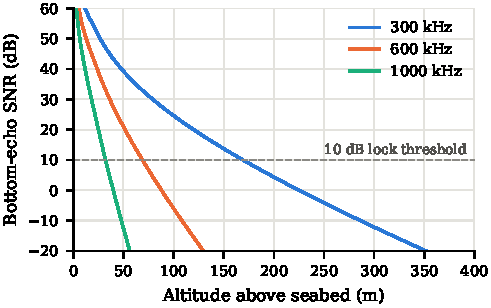
\includegraphics[width=\columnwidth]{fig/d3_bottomlock.pdf}
\caption{Bottom-echo SNR versus altitude at 3800~m depth for the assumed low-cost source level.}
\label{fig:d3}
\end{figure}

\subsection{Mission Error Budget}

A 1~m/s vertical descent is followed by a 1~h survey at 1.5~m/s (500~m legs, 50~m spacing), in 500 Monte Carlo runs. Above bottom-lock range, the vehicle navigates either on the INS alone, where error grows as $\tfrac12 b_a t^2$, or by DVL water-tracking, where the unknown current (Gauss--Markov in depth, $\sigma=0.1$~m/s, 300~m correlation length) integrates into position error. During the survey, heading error (bias plus heading-dependent deviation) and scale error add drift.

Fig.~\ref{fig:d4} gives the budget for 3800~m. Descent on a MEMS INS alone accumulates 51.6~km of error. Water-tracking reduces this to 200~m, and a 300~kHz unit that locks 137~m earlier improves it only to 193~m. At 6000~m the water-track descent error is 264~m. During the survey, a MEMS heading sensor ($1^\circ$ bias and deviation) adds 61~m, against 1.3~m for fibre-optic-grade heading. The descent, not the DVL, dominates: absolute position at the seabed requires acoustic positioning such as USBL or LBL.

\begin{figure}[t]
\centering
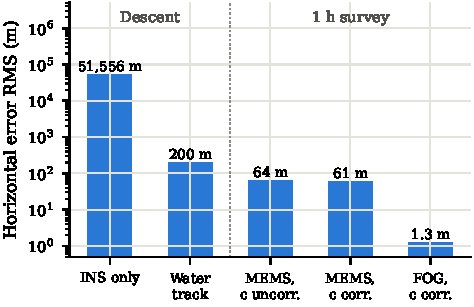
\includegraphics[width=\columnwidth]{fig/d4_budget.pdf}
\caption{Horizontal error budget for a 3800~m dive with a 1~MHz DVL (500 Monte Carlo runs, log scale).}
\label{fig:d4}
\end{figure}

\subsection{Pressure Housing versus Pressure Tolerance}

For a tube of inner radius $a$ and outer radius $b$ under external pressure $p$, the Lam\'e inner hoop stress gives the yield-limited pressure
\begin{equation}
p_y=\sigma_y\,\frac{b^2-a^2}{2b^2},
\end{equation}
and the Windenburg--Trilling formula~\cite{windenburg1934} gives the elastic buckling pressure of a tube of length $L$, diameter $D$ and wall $t$:
\begin{equation}
p_{cr}=\frac{2.42\,E\,(t/D)^{2.5}}{(1-\nu^2)^{0.75}\left[L/D-0.45\sqrt{t/D}\right]} .
\end{equation}
With safety factors of 1.5 on yield and 3 on buckling, an 80~mm bore, 200~mm long housing needs a 6.4~mm (3800~m) or 10.0~mm (6000~m) wall in 7075-T6 aluminium, or 5.2 and 6.3~mm in Ti-6Al-4V (Fig.~\ref{fig:d5}). Polycarbonate and acrylic cannot reach either depth; a typical 150~mm polycarbonate hobby-AUV tube with a 5~mm wall collapses at about 25~m.

The proposed alternative is a pressure-tolerant DVL: electronics fully potted in vacuum-degassed polyurethane or immersed in oil, with no electrolytic capacitors, no hollow-can crystals (a MEMS oscillator instead) and no relays, and a cable potted directly into the block. With no internal voids, no pressure difference acts across a wall. Liquid-filled power electronics have operated at 300~bar~\cite{pittini2011}; qualification of microcontroller-class boards at 380--600~bar remains to be done.

\begin{figure}[t]
\centering
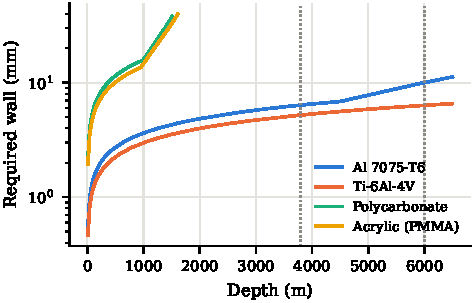
\includegraphics[width=\columnwidth]{fig/d5_wall.pdf}
\caption{Required wall thickness versus depth for an 80~mm bore, 200~mm long housing. Curves end where no wall thickness suffices.}
\label{fig:d5}
\end{figure}

\section{Discussion and Limitations}

The results define what a low-cost DVL must achieve and how its data should be fused. The most consequential design choice is the number of receive chains, which sets the deliverable noise (Table~\ref{tab:b5}) and with it the smallest detectable fault. Calibrating the fault detector requires no extra hardware, only the filter's own covariance.

The study has four limitations. First, all results are from simulation; the hardware of Section~\ref{sec:design} has not yet been built, and transducer ringing, cross-talk, receiver noise and multipath in tanks are not modelled. Second, the navigation model is translational; attitude is assumed known except for heading error in Section~\ref{sec:deep}. Third, the bottom-lock analysis depends on an assumed source level and seabed backscatter. Fourth, pressure tolerance is a design proposal, not a tested result.

\section{Conclusion and Future Work}

A four-beam, 1~MHz DVL built from commodity components is limited by speckle to about 0.07~m/s per ping, and can deliver 39--77~Hz Doppler noise at 5~Hz. Tightly coupled fusion still bounds position error to decimetres over a minute. Normalising beam residuals with the full innovation covariance makes fault detection consistent, removing a 30-fold false-alarm inflation, and a 2-of-3 quarantine rule prevents fault absorption. For deep operation, sound speed must be corrected, and the descent rather than the DVL limits navigation accuracy. Future work will build the DVL, measure its noise and range in a tank, and validate fault-tolerant navigation against encoder and GPS ground truth.

\section*{Acknowledgment}
The author used an AI assistant (Claude, Anthropic) for help with simulation code, analysis and language editing. All simulations were run and their results checked by the author.

\section*{Data Availability}
The simulation notebook that produces every figure and table in this paper is available from the author on request.

\begin{thebibliography}{99}
\bibitem{paull2014} L.~Paull, S.~Saeedi, M.~Seto, and H.~Li, ``AUV navigation and localization: A tutorial and review,'' \emph{IEEE J. Ocean. Eng.}, vol.~39, no.~1, pp.~131--149, 2014.
\bibitem{wl_a50} Water Linked AS, ``DVL A50,'' product page. [Online]. Available: \url{https://waterlinked.com/shop/dvl-a50-1248}. Accessed: Oct.~21, 2026.
\bibitem{tasman} Teledyne RD Instruments, ``Tasman DVL,'' datasheet. [Online]. Available: \url{https://teledynemarine.com/en-us/products/SiteAssets/RD\%20Instruments/Tasman_DVL.pdf}
\bibitem{catsamas2022} S.~Catsamas, B.~Shi, B.~Deletic, M.~Wang, and D.~T.~McCarthy, ``A low-cost, low-power water velocity sensor utilizing acoustic Doppler measurement,'' \emph{Sensors}, vol.~22, no.~19, art.~7451, 2022, doi:10.3390/s22197451.
\bibitem{tal2017} A.~Tal, I.~Klein, and R.~Katz, ``Inertial navigation system/Doppler velocity log (INS/DVL) fusion with partial DVL measurements,'' \emph{Sensors}, vol.~17, no.~2, art.~415, 2017, doi:10.3390/s17020415.
\bibitem{liu2018} P.~Liu, B.~Wang, Z.~Deng, and M.~Fu, ``INS/DVL/PS tightly coupled underwater navigation method with limited DVL measurements,'' \emph{IEEE Sensors J.}, vol.~18, no.~7, pp.~2994--3002, 2018, doi:10.1109/JSEN.2018.2800165.
\bibitem{yao2023} Y.~Yao, X.~Xu, X.~Xu, and I.~Klein, ``Virtual beam aided SINS/DVL tightly coupled integration method with partial DVL measurements,'' \emph{IEEE Trans. Veh. Technol.}, vol.~72, no.~1, pp.~418--427, 2023, doi:10.1109/TVT.2022.3204651.
\bibitem{klein2020} I.~Klein and Y.~Lipman, ``Continuous INS/DVL fusion in situations of DVL outages,'' in \emph{Proc. IEEE/OES Auton. Underwater Vehicles Symp. (AUV)}, 2020, doi:10.1109/AUV50043.2020.9267945.
\bibitem{klein2022} I.~Klein, Y.~Gutnik, and Y.~Lipman, ``Estimating DVL velocity in complete beam measurement outage scenarios,'' \emph{IEEE Sensors J.}, vol.~22, no.~21, pp.~20730--20737, 2022, doi:10.1109/JSEN.2022.3206310.
\bibitem{yona2023} M.~Yona and I.~Klein, ``MissBeamNet: Learning missing Doppler velocity log beam measurements,'' arXiv:2301.11597, 2023.
\bibitem{cohen2024} N.~Cohen and I.~Klein, ``Seamless underwater navigation with limited Doppler velocity log measurements,'' 2024, doi:10.1109/TIV.2024.3457772.
\bibitem{zhu2025} T.~Zhu, J.~Li, G.~Wan, and Y.~Sun, ``Research on error correction of beam fault in SINS/DVL tightly coupled navigation system,'' \emph{J. Phys.: Conf. Ser.}, vol.~3007, art.~012032, 2025, doi:10.1088/1742-6596/3007/1/012032.
\bibitem{yang2022} H.~Yang, X.~Gao, H.~Huang, B.~Li, and J.~Jiang, ``A tightly integrated navigation method of SINS, DVL, and PS based on RIMM in the complex underwater environment,'' \emph{Sensors}, vol.~22, no.~23, art.~9479, 2022, doi:10.3390/s22239479.
\bibitem{quartararo2022} J.~D.~Quartararo and S.~E.~Langel, ``Detecting slowly accumulating faults using a bank of cumulative innovations monitors in Kalman filters,'' \emph{NAVIGATION}, vol.~69, no.~1, 2022, doi:10.33012/navi.507.
\bibitem{blanford2018} T.~E.~Blanford, D.~C.~Brown, and R.~J.~Meyer, ``Design considerations for a compact correlation velocity log,'' \emph{Proc. Meetings Acoust.}, vol.~33, art.~070003, 2018, doi:10.1121/2.0000928.
\bibitem{rypkema2019} N.~R.~Rypkema, ``Underwater \& out of sight: Towards ubiquity in underwater robotics,'' Ph.D. dissertation, MIT/WHOI Joint Program, 2019.
\bibitem{mcphail2008} S.~McPhail, M.~Furlong, V.~Huvenne, and P.~Stevenson, ``Autosub6000: Results of its engineering trials and first science missions,'' National Oceanography Centre, Southampton, U.K. [Online]. Available: \url{https://nora.nerc.ac.uk/id/eprint/165904/}
\bibitem{liu2024} Y.~Liu, Y.~Sun, B.~Li, X.~Wang, and L.~Yang, ``Experimental analysis of deep-sea AUV based on multi-sensor integrated navigation and positioning,'' \emph{Remote Sens.}, vol.~16, no.~1, art.~199, 2024.
\bibitem{mackenzie1981} K.~V.~Mackenzie, ``Nine-term equation for sound speed in the oceans,'' \emph{J. Acoust. Soc. Am.}, vol.~70, no.~3, pp.~807--812, 1981.
\bibitem{francois1982} R.~E.~Francois and G.~R.~Garrison, ``Sound absorption based on ocean measurements. Part II: Boric acid contribution and equation for total absorption,'' \emph{J. Acoust. Soc. Am.}, vol.~72, no.~6, pp.~1879--1890, 1982.
\bibitem{barshalom2001} Y.~Bar-Shalom, X.~R.~Li, and T.~Kirubarajan, \emph{Estimation with Applications to Tracking and Navigation}. New York, NY, USA: Wiley, 2001.
\bibitem{windenburg1934} D.~F.~Windenburg and C.~Trilling, ``Collapse by instability of thin cylindrical shells under external pressure,'' \emph{Trans. ASME}, vol.~56, pp.~819--825, 1934.
\bibitem{pittini2011} R.~Pittini, M.~Hernes, and A.~Petterteig, ``Pressure tolerant power electronics for deep and ultra-deep water,'' in \emph{Proc. Offshore Technol. Conf. (OTC)}, Houston, TX, USA, 2011.
\end{thebibliography}

\end{document}
